\section{Combined reach projections}

The total reach of all 0.5~mm data only is shown in Figure~\ref{fig:reach0p5only}.

\begin{figure}[H]
  \centering
     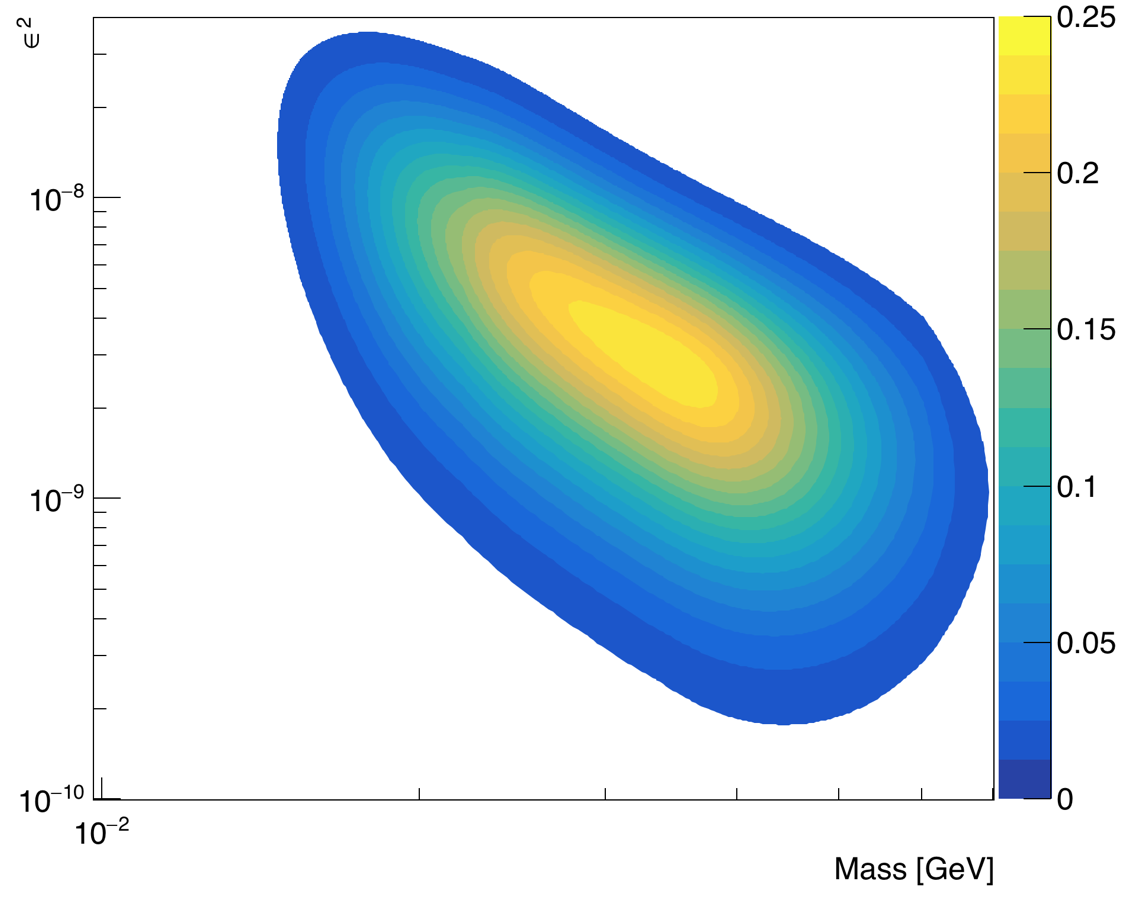
\includegraphics[width=0.8\textwidth]{plots/reachall_0p5.png}
  \caption{The expected signal yield for the full 100$\%$ dataset with all 0.5~mm data.}
  \label{fig:reach0p5only}
\end{figure} 

The reach as shown in Figure~\ref{fig:reach0p5only} uses the projected zCut for 100$\%$ of the data and assumes that we can optimize and use the L2L2 dataset. Using the same assumptions, we can obtain the reach for the 1.5~mm dataset alone in Figure~\ref{fig:reach1p5only}.

\begin{figure}[H]
  \centering
     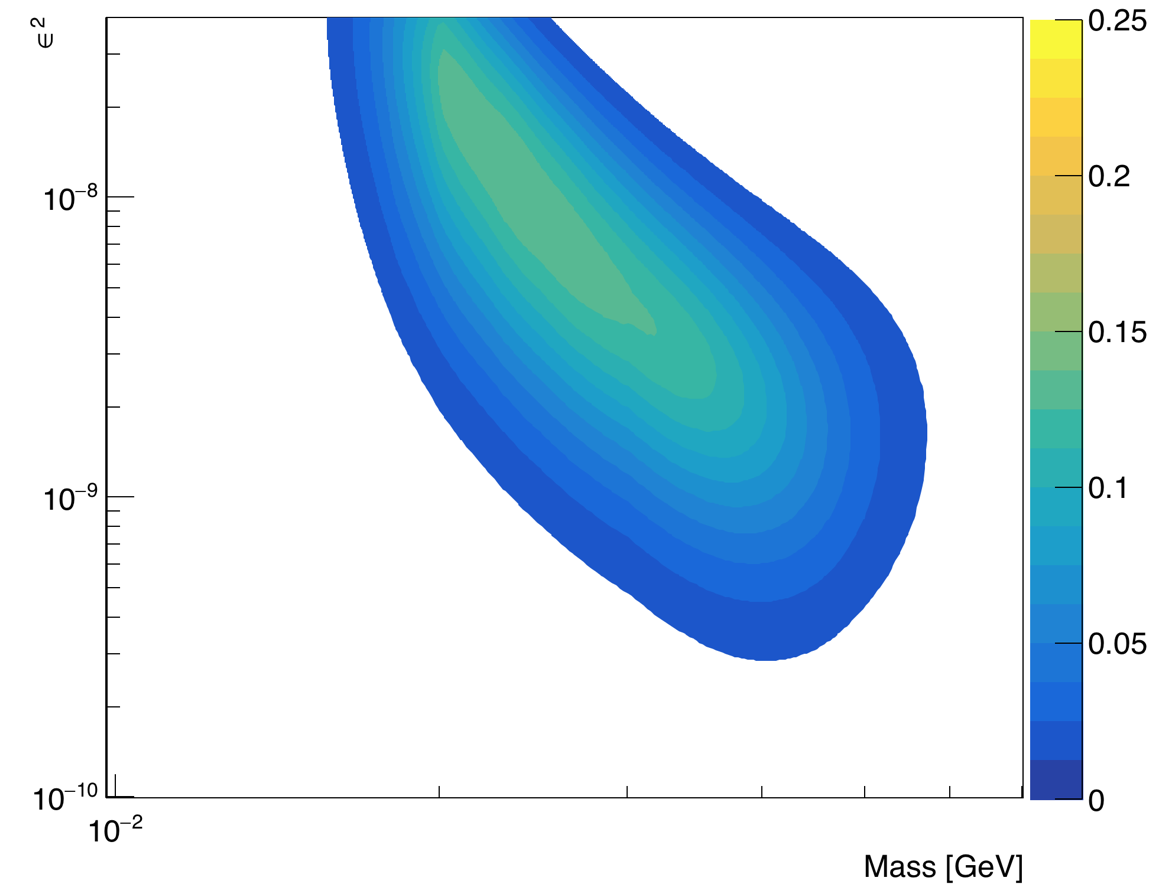
\includegraphics[width=0.8\textwidth]{plots/reachall_1p5.png}
  \caption{The expected signal yield for the full 100$\%$ dataset with all 1.5~mm data.}
  \label{fig:reach1p5only}
\end{figure} 

By combining the reach of the 0.5~mm and 1.5~mm datasets, we obtain the full upper limit of the reach we can expect when we unblind the full 2015 data as shown in Figure~\ref{fig:reachall}.

\begin{figure}[H]
  \centering
     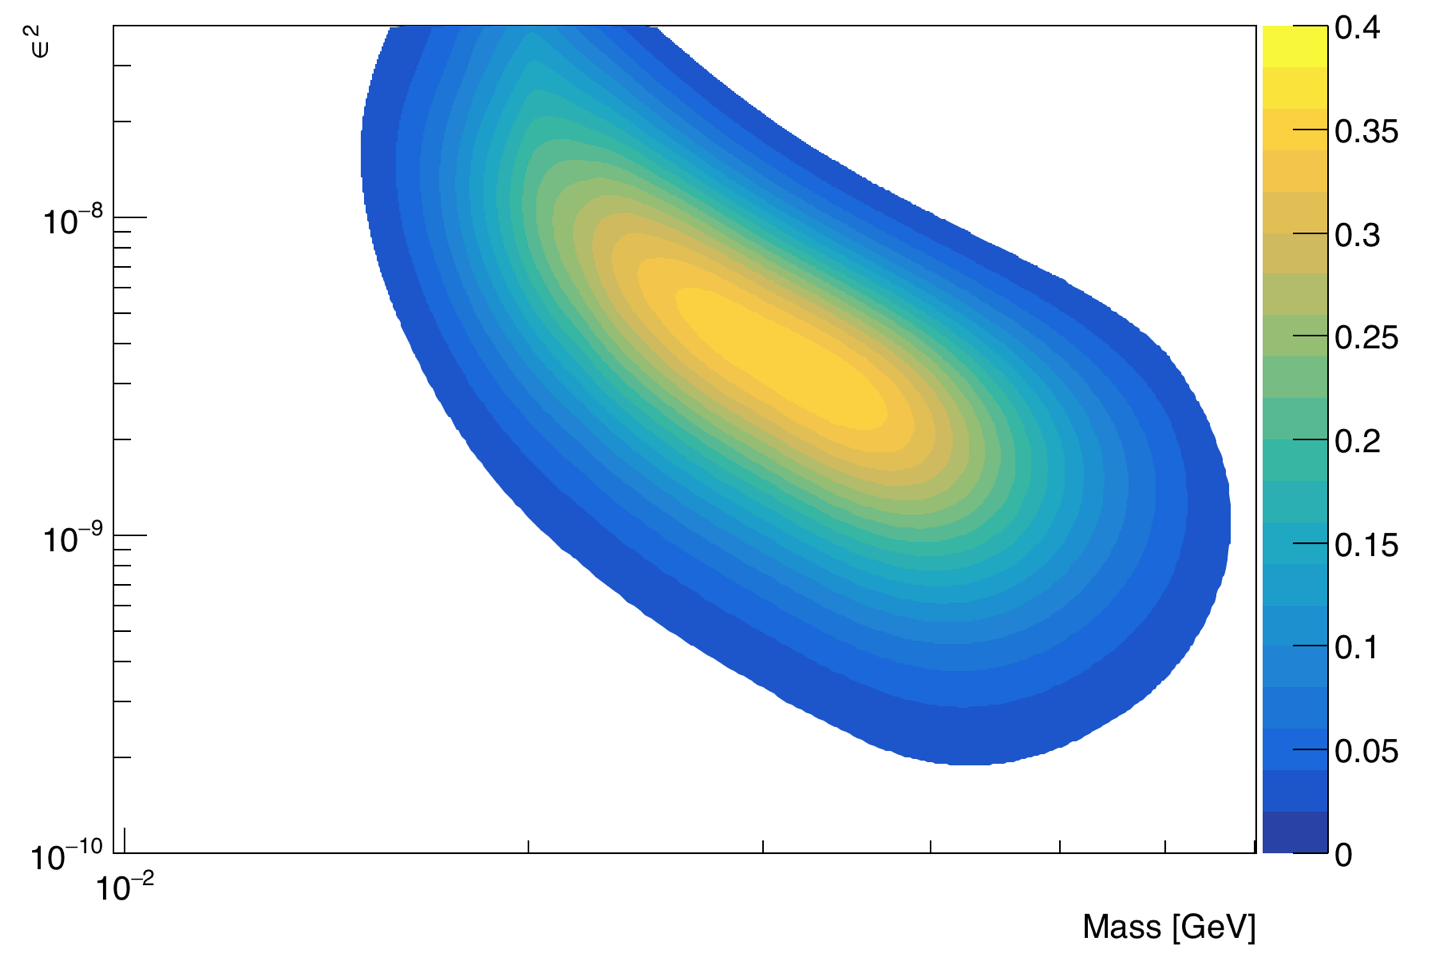
\includegraphics[width=0.8\textwidth]{plots/reachall.png}
  \caption{The expected signal yield for the full 100$\%$ dataset with 0.5~mm and 1.5~mm data combined.}
  \label{fig:reachall}
\end{figure} 

While the statistics of the 0.5~mm dataset drive the reach, the various settings of the SVT and different layer requirements can contribute to the reach by probing the parameter space in different regions of mass and coupling. The maximum signal in  Figure~\ref{fig:reachall} is 0.39~events. In order to have obtained any reach with the data, it would have been necessary to run an additional six times longer than what we did. 
\indent The contributions from the L2L2 datasets are upper limit estimates that require improved mass resolution and removal of high z backgrounds. 
